\documentclass[12pt]{article}
\oddsidemargin=0.0in
\evensidemargin=0.0in
\textwidth=6.5in
\topmargin=-0.55in
\textheight=9.3in
\usepackage{hyperref}
\usepackage{graphicx}

\begin{document}
\pagestyle{empty}
 
\begin{center}
{\LARGE {\bf Homework Five}}\\
\bigskip
{\Large {\bf Calculus I}}\\
\bigskip
{\Large {\bf College of the Atlantic}}\\
\bigskip
{ {\bf Due Friday, October 18, 2024}}\\ 
\end{center}
\medskip


\noindent There is one part to this assignment.\\

\noindent {\bf Part 1: WeBWorK}.  Do Homework 05A and 05B on
WeBWorK.  The WeBWorK page is here: 
\url{https://webwork-hosting.runestone.academy/webwork2/coa-feldman-es1024-fall2024/}.
I recommend doing the WeBWorK part of the homework first.  This will
enable you to benefit WeBWorK's instant feedback before you do part
two.\\ 


\noindent {\bf Part 2: Non-WeBWorK problems}.  Here are some
instructions for how to submit this part of the assignment.
\begin{itemize}
  \setlength{\itemsep}{0mm}
\item Do the problems by hand using pencil (or pen) and paper.
  There is no need to type this assignment.
%\item If you like working on a tablet, go for it. 
\item Make a pdf scan of your work using genius scan or some
  similar scanning app.  Please make the homework into a single
  pdf, not multiple pdfs.
\item Submit the assignment on google classroom.  Please don't
  email it to me.
  %(Between my two classes I will be receiving
  %around 60 assignments a week.  Keeping track of them all in email 
  %is challenging.)
\item If you want, you can do the non-WeBWorK problems in pairs and
  submit only one assignment for the two of you. \\
\end{itemize}


\noindent Here are some non-WeBWorK problems.


%\begin{figure}[h]
%\begin{center}
%\vspace{1mm}
%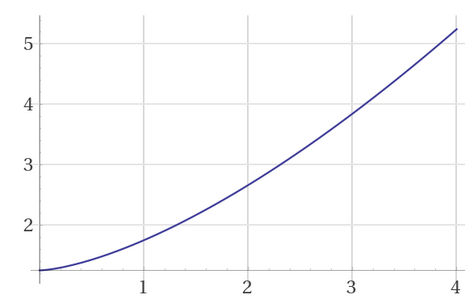
\includegraphics[width=3.0in]{graph_HW04_1.png}
%\vspace{-1mm}
%\caption{The position of a object (in meters) as a function of time
%  (in seconds). }
%\vspace{-5mm}
%\label{fig:graph1}
%\end{center}
%\end{figure}
%%\vspace{0mm}



\begin{enumerate}
\setlength{\itemsep}{8mm}


\item Let $g(x) = 1/x$.
  \begin{enumerate}
    \item Determine the equation of the line tangent to $g(x)$ at
      $x=1/2$.
    \item Make a plot of $g(x)$ and the tangent line you just
      found. (A sketch by hand is fine.)
  \end{enumerate}

\item A box of tofu is dropped off a tall building. The height of the
  tofu, in meters, is given by the function $h(t) = 100 - 9.8t^2$,
  where $t$ is measured in seconds.
  \begin{enumerate}
  \item What is the position of the tofu when $t=2$ seconds?
  \item What is the position of the tofu when $t=3$ seconds?
  \item What is the average speed of the tofu between $t=2$ and
    $t=3$ seconds?
  \item What is the speed of the tofu when $t=2$ seconds?
  \item What is the speed of the tofu when $t=3$ seconds?
  \end{enumerate}
  Be sure to include units with your answers. 
  
\end{enumerate}

\end{document}

  \setlength{\itemsep}{-1mm}
  \item Determine an equation for the linear function that generates
    the values in the table below.  

\begin{center}
\begin{tabular}{|| l | l ||}
\hline $x$ & $f(x)$ \\
\hline
5.2 & 27.8 \\
5.3 & 29.2 \\
5.4 & 30.6 \\
5.5 & 32.0 \\
5.6 & 33.4 \\
\hline
\end{tabular}
\end{center}





\end{document}
